\section{Implementation and Encountered Problems}

In this section, we present our implementation choices and compare them to discarded alternatives to justify them. 
We also describe what difficulties we encountered during development and how we addressed them.

\subsection{Syntax}

First, we formalize the abstract syntax of boolean formulas containing conjunctions, disjunctions, implications, and negations. 

\subsubsection{Abstract Syntax.}

We state an inductive definition of the type \texttt{form} with a set of constructors describing how to build up a formula:
\begin{equation}
    p, q ::= x\;|\;\texttt{true}\;|\;\texttt{false}\;|\;p \land q\;|\;p \lor q\;|\;p \rightarrow q\;|\;\neg p
\end{equation}

For identifiers, we introduce the type \texttt{id} with a single constructor \texttt{Id} that wraps a string. We also define an equality function comparing two identifiers and returning \texttt{true} if and only if their contained strings are equal. To ease proof development in the rest of the project, we prove some basic lemmas about the function by case distinction, namely \emph{reflexivity}, \emph{equivalence with propositional equality}, and \emph{decidability} of equality of identifiers.

\subsubsection{Concrete Syntax.}

To make reading and writing formulas easier, we use \textsc{Coq}'s \texttt{Notation}s system, as well as a \texttt{Coercion} from an identifier as a formula. 
The main difficulty lies in assigning precedence levels to the individual constructors that pay respect to the commonly assumed binding of operators. 
Given the \emph{binds stronger} relation ($>$), that is:
\begin{equation}
    \neg > \land > \lor >\,\rightarrow
\end{equation}
For example, $x \lor \neg y \land z \rightarrow \texttt{false}$ is interpreted as $(x \lor ((\neg y) \land z) \rightarrow \texttt{false}$. 

\subsection{Semantics}

Now that we can write a formula in \textsc{Coq}, we want to define its semantics, i.e., if we interpret it as \texttt{true} or \texttt{false}.

\subsubsection{Valuations.}

To do so, we need to know which boolean values to replace all identifiers occurring in a formula with.
Therefore, we define the type \texttt{valuation}. 
A \emph{valuation} is a function that, being passed an identifier, returns \texttt{true} or \texttt{false}, or, in other words, a valuation is a total map from identifiers to booleans. 
Our implementation is analogous to the total map defined by Pierce et al. in \cite{pierceSF}.
% An empty valuation is a valuation that returns \texttt{false} for all arguments.

Again, to simplify writing and reading valuations, we introduce a \texttt{Notation} \texttt{x !-> b ;; v} to override a valuation \texttt{v} with a new value \texttt{b} for \texttt{x}. 
At first, we used just a single semicolon, but this caused conflicts with list notations. 

We also specify some lemmas of \cite{pierceSF} for later reasonings. 
Their proofs rely on the functional extensionality axiom, stating that two functions are equal if and only if their applications to all their possible arguments are equal. 
It is known to be compatible with \textsc{Coq}'s logical core.

\subsubsection{Interpreter.}

The \texttt{valuation} type allows us to define a recursive interpretation function \texttt{interp}.
Applied to a valuation and a formula, it returns \texttt{true} if and only if the formula holds by traversing a formula bottom-up and pattern matching on it.
All the necessary functions, such as \texttt{andb}, \texttt{orb}, and \texttt{negb} are already implemented in \textsc{Coq}. 
They even suffice to compute the result of an implication since $p \rightarrow q$ is known to be equivalent to $\neg p \lor q$.

\subsection{Optimizer}

Sometimes, a formula's interpretation can be derived or, at least, simplified on a purely syntactical level, leaving it in a form that is easier to read and reducing the computation effort needed by the interpretation function while preserving the semantics.
In this part of the project, we therefore introduce an optimization function \texttt{optim}.

\subsubsection{Minimality.}

A key challenge was formally defining what a simplification is and what property the result of \texttt{optim} should have.

A \emph{simplification} reduces the applications of the binary operators $\land$, $\lor$ and $\rightarrow$ to one of their two arguments or an \emph{atom}, i.e., the boolean values \texttt{true} and \texttt{false}. 
Additionally, when applied to an atom, the unary operation $\neg$ can be simplified to an atom.

The aim is to leave a formula $p$ in a form that cannot be simplified further on a syntactical level.
We assume this to be the case in exactly two mutually exclusive situations:
\begin{itemize}
    \item $p$ is an atom, or
    \item $p$ does not contain any atoms.
\end{itemize}
When one of the situations applies, we say $p$ is in \emph{minimal form}. Formalizing this definition in \textsc{Coq}, we require either a fixpoint returning \texttt{true} if and only if a formula does not contain atoms or an inductive proposition.
While we initially opted for a fixpoint, proving the correctness of our optimizer later turned out easier with an inductive proposition. 
A formula does not contain an atom if it is an identifier or if all its subformulas do not contain atoms.

We settle on a set of laws that our optimizer uses and allow it to fulfill the above-mentioned correctness and minimality requirements:
\begin{alignat}{4}
    \texttt{true} \land p &\equiv p &p \land \texttt{true} &\equiv p &\texttt{false} \land p &\equiv \texttt{false}\hspace*{20pt}&p \land \texttt{false} &\equiv \texttt{false} \\
    \texttt{true} \lor p &\equiv \texttt{true}\hspace*{20pt}&p \lor \texttt{true} &\equiv \texttt{true}\hspace*{20pt}&\texttt{false} \lor p &\equiv p &p \lor \texttt{false} &\equiv p \\
    \texttt{true} \rightarrow p &\equiv p &p \rightarrow \texttt{true} &\equiv \texttt{true} &\texttt{false} \rightarrow p &\equiv \texttt{true} &p \rightarrow \texttt{false} &\equiv \neg p \\
    &&\neg \texttt{true} &\equiv \texttt{false} &\neg \texttt{false} &\equiv \texttt{true}
\end{alignat}

\subsubsection{Implementation.}

The actual implementation of the optimizer in \textsc{Coq} requires a bit of thought.
Indeed, our first implementation attempt was a top-down traversal of the abstract syntax tree of the given formula and successive application of the listed simplifications.
However, this misses some optimization potential as it may only become available after optimizing subformulas.
To try and remedy this, we wrote a recursive function repeatedly applying \texttt{optim} on a formula until reaching a fixpoint.
While a fixpoint is eventually reached in practice, \textsc{Coq} cannot know and rejects the function as new arguments to \texttt{optim} are not obviously smaller.

\begin{figure}[t]
    \centering
    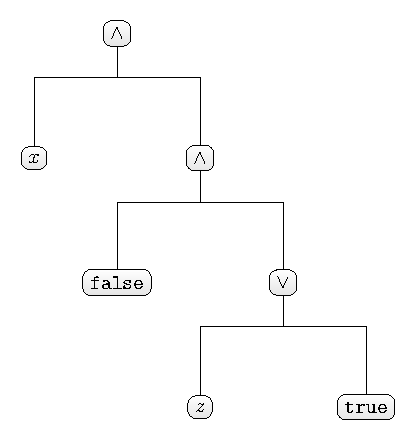
\includegraphics[scale=0.82,valign=t]{figures/optimizer1.pdf}
    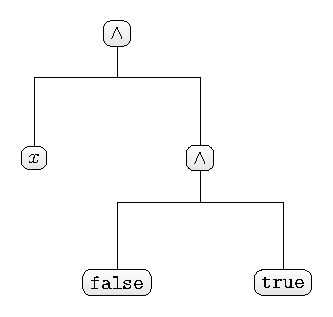
\includegraphics[scale=0.82,valign=t]{figures/optimizer2.pdf}
    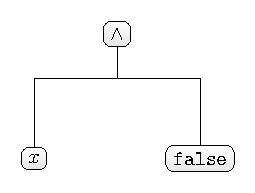
\includegraphics[scale=0.82,valign=t]{figures/optimizer3.pdf}
    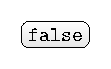
\includegraphics[scale=0.82,valign=t]{figures/optimizer4.pdf}
    \caption{Successive syntactical optimization steps on $x \land (\texttt{false} \land (z \lor \texttt{true}))$.}
    \label{fig:optimizer}
\end{figure}

Instead, our revised approach only traverses the passed formula once and hence only requires linear runtime.
We achieve this by performing a post-order depth-first-search (DFS) on the abstract syntax tree of the passed formula.
This way, optimizations of subformulas are directly taken into account.
Even though sometimes it is sufficient to simplify only one or even no subformula, we always traverse the whole tree for easier proving of the required properties.
Figure \ref{fig:optimizer} illustrates such a case, where for the formula $x \land (\texttt{false} \land (z \lor \texttt{true}))$, the subformula $z \lor \texttt{true}$ is simplified to \texttt{true} first, even though $\texttt{false} \land (z \lor \texttt{true})$ could directly be simplified to \texttt{false} from the get-go.
Note, however, that the formula is translated to \texttt{false} without even running the interpreter just by its syntax.

\subsubsection{Properties.}

To close off this section, we must formally verify that our optimizer truly meets its requirements.
First and foremost, the following theorem holds:
\begin{theorem}
    For all valuations $v$ and formulas $p$, $\texttt{interp}\;v\;p = \texttt{interp}\;v\;(\texttt{optim}\;p)$, i.e., the optimizer is correct since it preserves the semantics of formulas.
\end{theorem}
\begin{proof}
    We proceed by induction on the structure of $p$. 
    The non-trivial cases $p = q_1 \land q_2$, $p = q_1 \lor q_2$ and $p = q_1 \rightarrow q_2$ are all shown by case distinction on $\texttt{optim}\;q_1$ and $\texttt{optim}\;q_2$ and application of the induction hypotheses claiming the optimizer is correct for $q_1$ and $q_2$.
    $p = \neg q$ follows the same pattern for a single subformula $q$. \qed
\end{proof}
The main challenges for formally proving this theorem in \textsc{Coq} do not lie in the reasoning but rather in removing redundancies.
Consequently, as for many other proofs of the project, we decided to first write a mostly manually written version before looking out for automation potential.
In a final step, we filtered out common patterns through custom tactics through the \texttt{Ltac} language. 

We also prove this second theorem to show our optimizer is actually exhaustive:
\begin{theorem}
    For all formulas $p$, the result of the optimizer $\texttt{optim}\;p$ is in minimal form.
\end{theorem}
\begin{proof}
    We proceed by induction on the structure of $p$.
    For the cases $p = q_1 \land q_2$, $p = q_2 \lor q_2$, $p = q_1 \rightarrow q_2$ and $p = \neg q$, we perform case distinctions on the induction hypotheses (minimality of the subformulas), as well as the results of the optimizer applied to them.
    If necessary, we invert the induction hypotheses involving the deconstructed optimizer results.
    Then, it follows directly from the hypotheses set that $p$ either does not contain atoms or, on the contrary, is an atom. \qed
\end{proof}
For this \textsc{Coq} proof, many cases are very similar, but, e.g., differ in the actual atom $p$ is equal to, reducing the potential for automation, as one must carefully introduce a fitting witness for the left branch of minimality, i.e., \texttt{exists b, p = form\_bool b}.
Nevertheless, we factor out the recurrent patterns of deconstructing and rewriting with the induction hypotheses and destructing $\texttt{optim}\;q$ for a subformula $q$ and then inverting one of the induction hypotheses. In some rare cases, some forms are shelved in the process, requiring the use of \texttt{Unshelve}, which we were unaware of beforehand.

\subsection{Solver}

% difficulty: even though cases pretty similar, always slight changes, need to consider existential closely
% don't know why unshelving needed, where shelved originally

\subsection{A Subsection Sample}
Please note that the first paragraph of a section or subsection is
not indented. The first paragraph that follows a table, figure,
equation etc. does not need an indent, either.

Subsequent paragraphs, however, are indented.

\subsubsection{Sample Heading (Third Level)} Only two levels of
headings should be numbered. Lower level headings remain unnumbered;
they are formatted as run-in headings.

\paragraph{Sample Heading (Fourth Level)}
The contribution should contain no more than four levels of
headings. Table~\ref{tab1} gives a summary of all heading levels.

\begin{table}
\caption{Table captions should be placed above the
tables.}\label{tab1}
\begin{tabular}{|l|l|l|}
\hline
Heading level &  Example & Font size and style\\
\hline
Title (centered) &  {\Large\bfseries Lecture Notes} & 14 point, bold\\
1st-level heading &  {\large\bfseries 1 Introduction} & 12 point, bold\\
2nd-level heading & {\bfseries 2.1 Printing Area} & 10 point, bold\\
3rd-level heading & {\bfseries Run-in Heading in Bold.} Text follows & 10 point, bold\\
4th-level heading & {\itshape Lowest Level Heading.} Text follows & 10 point, italic\\
\hline
\end{tabular}
\end{table}


\noindent Displayed equations are centered and set on a separate
line.
\begin{equation}
x + y = z
\end{equation}
Please try to avoid rasterized images for line-art diagrams and
schemas. Whenever possible, use vector graphics instead (see
Fig.~\ref{fig1}).

\begin{figure}
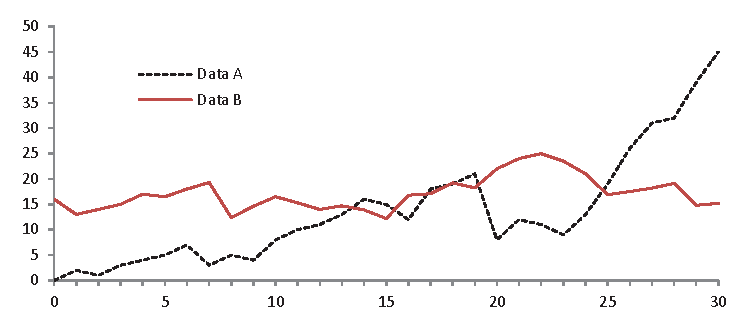
\includegraphics[width=\textwidth]{fig1.eps}
\caption{A figure caption is always placed below the illustration.
Please note that short captions are centered, while long ones are
justified by the macro package automatically.} \label{fig1}
\end{figure}

\begin{theorem}
This is a sample theorem. The run-in heading is set in bold, while
the following text appears in italics. Definitions, lemmas,
propositions, and corollaries are styled the same way.
\end{theorem}
%
% the environments 'definition', 'lemma', 'proposition', 'corollary',
% 'remark', and 'example' are defined in the LLNCS documentclass as well.
%
\begin{proof}
Proofs, examples, and remarks have the initial word in italics,
while the following text appears in normal font.
\end{proof}